% $Id: template.tex 11 2007-04-03 22:25:53Z jpeltier $

\documentclass{vgtc}                          % final (conference style)
%\documentclass[review]{vgtc}                 % review
%\documentclass[widereview]{vgtc}             % wide-spaced review
%\documentclass[preprint]{vgtc}               % preprint
%\documentclass[electronic]{vgtc}             % electronic version

%% Uncomment one of the lines above depending on where your paper is
%% in the conference process. ``review'' and ``widereview'' are for review
%% submission, ``preprint'' is for pre-publication, and the final version
%% doesn't use a specific qualifier. Further, ``electronic'' includes
%% hyperreferences for more convenient online viewing.

%% Please use one of the ``review'' options in combination with the
%% assigned online id (see below) ONLY if your paper uses a double blind
%% review process. Some conferences, like IEEE Vis and InfoVis, have NOT
%% in the past.

%% Figures should be in CMYK or Grey scale format, otherwise, colour 
%% shifting may occur during the printing process.

%% These few lines make a distinction between latex and pdflatex calls and they
%% bring in essential packages for graphics and font handling.
%% Note that due to the \DeclareGraphicsExtensions{} call it is no longer necessary
%% to provide the the path and extension of a graphics file:
%% \includegraphics{diamondrule} is completely sufficient.
%%
\ifpdf%                                % if we use pdflatex
  \pdfoutput=1\relax                   % create PDFs from pdfLaTeX
  \pdfcompresslevel=9                  % PDF Compression
  \pdfoptionpdfminorversion=7          % create PDF 1.7
  \ExecuteOptions{pdftex}
  \usepackage{graphicx}                % allow us to embed graphics files
  \DeclareGraphicsExtensions{.pdf,.png,.jpg,.jpeg} % for pdflatex we expect .pdf, .png, or .jpg files
\else%                                 % else we use pure latex
  \ExecuteOptions{dvips}
  \usepackage{graphicx}                % allow us to embed graphics files
  \DeclareGraphicsExtensions{.eps}     % for pure latex we expect eps files
\fi%

%% it is recomended to use ``\autoref{sec:bla}'' instead of ``Fig.~\ref{sec:bla}''
\graphicspath{{figures/}{pictures/}{images/}{./}} % where to search for the images

\usepackage{microtype}                 % use micro-typography (slightly more compact, better to read)
\PassOptionsToPackage{warn}{textcomp}  % to address font issues with \textrightarrow
\usepackage{textcomp}                  % use better special symbols
\usepackage{mathptmx}                  % use matching math font
\usepackage{times}                     % we use Times as the main font
\renewcommand*\ttdefault{txtt}         % a nicer typewriter font
\usepackage{cite}                      % needed to automatically sort the references
\usepackage{tabu}                      % only used for the table example
\usepackage{booktabs}                  % only used for the table example
%% We encourage the use of mathptmx for consistent usage of times font
%% throughout the proceedings. However, if you encounter conflicts
%% with other math-related packages, you may want to disable it.


%% If you are submitting a paper to a conference for review with a double
%% blind reviewing process, please replace the value ``0'' below with your
%% OnlineID. Otherwise, you may safely leave it at ``0''.
\onlineid{0}

%% declare the category of your paper, only shown in review mode
\vgtccategory{Research}

%% allow for this line if you want the electronic option to work properly
\vgtcinsertpkg

%% In preprint mode you may define your own headline.
%\preprinttext{To appear in an IEEE VGTC sponsored conference.}

%% Paper title.

\title{Virtual Environment for Memorization and Content Exploration in Educational Settings}

%% This is how authors are specified in the conference style

%% Author and Affiliation (single author).
\author{Luke Grove\thanks{e-mail: grovee@colostate.edu}}
\affiliation{\scriptsize Undergraduate Student}

%% Abstract section.
\abstract
{
The prototype developed in this paper is designed to gauge how effective virtual environments are at facilitating content memorization, specifically with the context of education. Participants engage in a series of levels within a virtual environment and answer questions relating to a specific subject, and are then tested on their net memorization. Testing of the prototype shows that, despite initial flaws with orientation, participants quickly grow acclimatized to the format. Exposure to the prototype increase net memorization by 3.77 out of 10 points. The relative mean time of each level has an average decrease of 67.69 in between each level, although the observed error has an increase of 1.00 that potentially stems from influences of the environment on the learning process. %
} 
% end of abstract

%% ACM Computing Classification System (CCS). 
%% See <http://www.acm.org/class/1998/> for details.
%% The ``\CCScat'' command takes four arguments.

\CCScatlist{ 
%%  \CCScat{K.6.1}{Management of Computing and Information Systems}%
%%{Project and People Management}{Life Cycle};
%%  \CCScat{K.7.m}{The Computing Profession}{Miscellaneous}{Ethics}
    \CCScat{}{Human Computer Interaction, Virtual Environments, Memorization, Immersion, Education}{}{}
}

%% Copyright space is enabled by default as required by guidelines.
%% It is disabled by the 'review' option or via the following command:
% \nocopyrightspace

%%%%%%%%%%%%%%%%%%%%%%%%%%%%%%%%%%%%%%%%%%%%%%%%%%%%%%%%%%%%%%%%
%%%%%%%%%%%%%%%%%%%%%% START OF THE PAPER %%%%%%%%%%%%%%%%%%%%%%
%%%%%%%%%%%%%%%%%%%%%%%%%%%%%%%%%%%%%%%%%%%%%%%%%%%%%%%%%%%%%%%%%

\usepackage{graphicx}

\begin{document}

%% The ``\maketitle'' command must be the first command after the
%% ``\begin{document}'' command. It prepares and prints the title block.

%% the only exception to this rule is the \firstsection command
%%\firstsection{Introduction}

\maketitle

\section{Introduction} %for journal use above \firstsection{..} instead
There exists a wide variety of tools for the education of individuals, whether through word of mouth or written text. Computing technology has provided a similar avenue for the assimilation of information, and spurred on an expansive number of creative means for users to become more familiar with certain topics. However, there remain aspects of the field that have yet to be extensively analyzed through the lens of education, one of the more prominent outliers being virtual environments. While such interactive mediums have experienced much innovation over the past few decades, a way for users to effectively utilize the medium for learning has yet to become widespread in many settings, especially those where access to specialized equipment is limited. 

\subsection{Motivation}

Referencing personal experience as a university student, many students have access to a wide array of education-oriented tools to aid in the study of a variety of subjects. While effective, many of these boil down to writing down important pieces of text from course material, or simple memorization games [10]. Only a small fraction of these available resources attempt to make use of advances in augmented reality, virtual environments, or a realm of other interactive mediums. Yet, even these  do not fully commit to the medium [10]. If pupils were to have access to academic applications that utilize such immersive means they may see a benefit in their daily scholarly work. And so, this experiment is designed to explore what an application such as that would look like, and if it would provide a legitimate benefit to an individual's studies. 

Taking steps to further the field of education is important as more technology becomes available, so that students and others can become better familiar with advanced topics more quickly. Everyone learns differently, and if experiments such as the one set out in this document can provide the means for those who may not benefit from more traditional educational techniques, then the field would see improvement in the long term. It would be a missed opportunity to not exploit the possibilities presented by such a vast and interactive medium.

\subsection{Overview}

Through the lens of human computer interaction, the goal of this research is to develop an educational program that utilizes a virtual environment, and study how it may enhance the memorization of subject matter compared to more traditional methods. Subsequent experimentation will produce a study in which participants are tasked with taking a number of quizzes within this virtual environment for the sake of assessing net memorization of content in the context of an educational setting. The original ideas for the prototype are briefly described in this section, followed with a review of related work on computer-aided memorization, including concepts with augmented reality. A redesign of the original prototype is then elaborated upon along with details of a user study to test the prototype.

The prototype was originally planned around use of an augmented reality technology. This would have been designed using a version of Unity and the various AR packages supported on the software for deployment onto a smartphone. However, this presented several potential problems. A primary concern was that this would present too much of a deviation from learning applications people may be familiar with, and did not take advantage of the level of familiarity samples may have with other mediums, such as virtual environments. Similarly, participants may not have smartphones capable of supporting highly complex applications, or even possess smartphones at all. However, the operating systems of those that did own sufficiently capable smart phones would likely vary greatly, again spurring technical difficulties. This too caused some concerns about the integrity of data collection across several different platforms. A static approach was ultimately decided upon, as explained with the user study.

The prototype and the research born of it will \textbf{contribute} to the field of computer-aided memorization, but more specifically to how individuals and groups can utilize said technology in study techniques and educational settings.

\section{Related Work}

\subsection{Augmented Reality}

Prior research on education in the domain of augmented reality (AR) has investigated the impact of interactive features on memorization performance.

In 2018, Ahmad et al. [1] presented a preliminary analysis in which hearing impaired students engaged with an augmented reality prototype to aid in the memorization of elements of the Quran, the central religious text of Islam. This qualitative study highlighted how an AR interface was ideal for impaired users, but more importantly for present research, indicates that some level of immersion in AR was effective for memorization. A subsequent study by Musliza et al. [6] in 2021 released their work on the EzHifz application, another AR prototype meant to educate users on the Quran that utilized games users could engage in with varying referents. Their findings revealed that, through the VARK (visual, auditory, reading/writing, and kinesthetic) learning style, the application displayed promise as a tool for individuals to independently study the Quran and retain any learned content through memorization, as well as a way of improving user motivation. A visualization of the application is available in Figure 1, showing its user interface along with prompts and images visible on the memorization menu.

\begin{figure}[tb]
 \centering 
 
\includegraphics[width=\linewidth]{ezhifz.png}
 \caption{Screen-capture of the "EzHifz" application, showing the memorization menu. The image is from source \cite{src1}.}
 \label{fig:sample}
\end{figure}

Elements from these prior works, although primarily the subject matter, play a key role in the learning metric of the prototype. But while important, the applications described in these studies differ to this prototype in respect to their use of virtual environments. Specifically, while differing referents and types of motion played large roles in the memorization process, they lack any sort of environment generated around the user, or one that the user could otherwise immerse themselves in outside of a simple user interface.

\subsection{Virtual Reality and Immersion}

Preceding work on virtual reality (VR) technology has yielded a number examples of applications used for training purposes in work environments, such as in vehicle design or the visualization of important three-dimensional structures [6].

Previous research in 2010 by Ragan et al. [8] explores the impact of user immersion on memorization further by performing a study in which participants performed actions in a virtual environment through the use of head mounted displays (HMDs) in a virtual reality setup. In relation to memorization performance, the study showed that even slight increases in user immersion were associated with significant increases in user task performance and attribute this to enhanced spatial cues. In discussing their findings, Ragan et al. admit it is not known if such levels of immersion would be necessary for education compared to more traditional display types, which may be just as effective. Nevertheless, they do not discount the clear educational advantages conferred by a virtual environment, and hypothesize the medium would become more practical with time. This aligns with the motivation behind the development of the prototype, which places importance on spacial cues within the virtual environment.

In an extension of this preceding study, in 2013 Hafner et al. [4] utilized two immersive means to explore the impact motion specifically has on memorization performance, along with the role immersion plays in that metric; the first and most immersive means was a Cave Automatic Virtual Environment (CAVE) format that involved extended reality (ER) technology; the second and less immersive was a desktop virtual environment that lacked any form of stereo vision. The team found no statistical proof that memorization performance varied with the motion type in their virtual environments, but speculate that part of this finding may stem from issues with popularity of the technology, as only a third of the users had any prior experience with either the CAVE format, whereas a much higher percentage had some level of familiarity with virtual motion and navigation. Contrary to Ragan et al., Hafner et al. found that memorization performance was not affected by immersion, but again attribute the cause of this to unfamiliarity with the CAVE system. 

From these contradictory findings it could be speculated that format too plays a role in the memorization process, along with how familiar participants are with it. If full-scale virtual environments are indeed impractical, or even not much more beneficial than more traditional educational formats, then less immersive means such as those explored by Hafner et al. might strike an efficient compromise between the two mediums. As the prototype utilizes a virtual environment on a desktop application, it is anticipated this pitfall with unfamiliarity is avoided.

\subsection{Virtual Environments}

Contrasted with AR and VR, there has been a lot more time to study the impact and effect that computer games, and through them virtual environments, have had on individuals.

A prior report in 2003 by Dyck et al. [2] explored the novel elements and approaches used in video games in order to assess their usefulness in more conventional applications. Of the beneficial aspects they discovered, the fluid way in which humans and the system interacted with each other is noted in particular. Through things such as subtle visual and audio clues, and context-aware view behaviors, the researchers speculate that user performance in regular work-spaces could see a benefit. While such features have largely become commonplace in today's online world, further research into the domain has yielded valuable insights. Components identified in this study are featured in this prototype, with a response UI and key visual elements.

In a study conducted much later in 2012, Koutsabasis et al. [5] developed a human-computer-interaction pedagogy that tested how virtual environments and other related technologies together with problem-based learning would effect the learning rates of students, along with their attitudes. In all, they found that the creative freedom the virtual environments facilitated had a significant impact on student performance and engagement despite some minor issues with the specific software they used. They went on to speculate that an immersive virtual environment application of similar means may yield similar benefit for many students, yet this notion required further testing in an empirical evaluation. While the methodologies used in the prototype do not replicate the exact learning methodologies of either Ahmad et al. or Koutsabasis et al. [1, 5], they are key considerations for the sake of education in the domain.

Similar to both AR and VR, immersion and motion are major factors in virtual environments that play into the memorization process. Preceding research in this regard is evident in a study by Pasch et al. [7] in 2009 that identifies four movement specific features (natural control, mimicry of movements, proprioceptive feedback, and physical challenge) for further investigation. These movement categories directly play into the immersion of the participants, as when their avatar within the virtual environment mimics dictated actions or suffers harm it was reported that participants became emotionally engaged with associated applications, expressing empathy for their representative body within the virtual environment. Parallel to this observation, specifically with the last movement type stipulated, it was noted that a physical challenge offered another convincing avenue of engagement and immersion for the participants. The prototype presents a number of physical challenges to its participants related to progression within the virtual environment.

Relating to memorization performance, a prior study in 2003 by Squire [9] analyses how video games (and through them, virtual environments) can be used in educational settings. In his report, he notes that despite the presence of a relevant games and simulations that are applicable to a wide array of content, very little empirical study had been performed on the subject at the time. He goes on to suggest specific genres and applications that would be pertinent for educators, some of which share similarities with the prototype elaborated upon later.

\subsection{Video Games and Concerns}

A paper published later on in 2007 by Gros [3] reiterates that, despite potential, video games (and associated virtual environments) are not the solution to education problems. Gros instead advocates for harnessing the most potent interactive elements of virtual environments and combining them with the pre-existing educational multimedia format in use today, and goes on to explain a number of approaches and considerations when adopting elements from virtual environments into educational formats. Both teachers and students are assigned different pedagogic roles in this explanation, along with developers themselves as this complex learning medium is tackled. In a study issued in 2015, Waddington [11] shares the same temperance as Gros in regards to the adoption of virtual environments in the classroom, but makes an effort to address potentially antiquated concerns from prior studies about the topic. While new ideas are brought forward relating to how far the medium had progressed in recent decades, new challenges are identified about virtual environment simulations specifically as perhaps shaping users to think in a strictly logical manner. Aligning with the motivation behind the development of the prototype, it is hoped that it is able to take forward some of the more positive views elaborated upon by Waddington while remaining cautious to the fundamental problems presented by the format, as described by them and Gros.

\section{Methodology}

\subsection{Participants}

The study consisted of nine volunteers (8 male, 1 female) and were 19-21 years old (mean=20.33, std-dev=0.82). Participants were recruited via word of mouth. All participants reported normal or corrected to normal vision. Five participants reported having a religious background, whereas only two reported that they actively practice a religion. Three reported any familiarity with the religion of Islam, all either majoring in history or computer science. Two participants reported having the same major (computer science), the other participants having unique fields of study. All nine participants reported having prior familiarity with virtual environments. Four of those participants reported using applications that contain virtual environments over 15 hours weekly, the rest were 3-5 hours weekly.

\subsection{Apparatus}

The software for this experiment was designed using Unity 2021.2.17 and the 3D Core preset, and will utilize in-engine scripts to generate any needed quantitative data during the study. Randomness in either format was set to the seed 54. This was performed on a Windows 10 home computer with an AMD Ryzen 7 3700X Matisse 3.6GHz 8-Core AM4 processor and an Nvidia GeForce RTX 3070 graphics card. All technical details relating to the creation of this software are present on a GitHub repository that has stored code, version history, and progress checkpoints of the software along with miscellaneous files.

\subsection{Procedure}

Before beginning the experiment informed consent was obtained from each participant, including acquiring their permission to record their screen during the testing of the prototype. Only a few participants had their screens recorded.

Testing for this experiment relied upon on a sample population of nine students at Colorado State University to measure the effectiveness of the prototype. In order to ensure the integrity of the study, a topic that these participants are unfamiliar with was needed so that there is no risk of bias coming into the experiment. More importantly, the materials they were to learn for this experiment should ideally not have been connected to their diverse fields of study, including psychology and computer science. And so, referencing prior work [1,6], the application attempted to educate the participants on certain elements of the Quran, along with the role motion plays with users who are familiar with immersive technology [4,8], incorporating elements from similar pedagogic experiments and other analyses performed within virtual environments [2,5]. This also allowed for a certain degree of continuity from these aforementioned studies, which also elaborate on computer aided memorization on this specific topic.

To verify the integrity of the results, after acquiring informed consent, each participant was administered an identical questionnaire that inquired about their gender, age, visual acuity, religious background, major, prior experience with virtual environments, and weekly use of applications that contain virtual environments. The practiced faith of each participant was not an incredibly significant measure in regards to much of the experiment, but their relation to Islam is an important qualifier that may affect their performance. The latter two items, additionally, are important as even if the content each individual is being quizzed on is completely unknown to them, some may acclimate to this virtual environment differently than a baseline sample and could alter the output data. However, given the widespread nature of interactive mediums like video games, it was anticipated that most users in the predicted age group will at least have some middling background with the format.

To formally begin the study, each participant took a ten question quiz on the Quran in order to gauge their initial understanding of the content. Questions for this quiz were randomly selected by the researcher from a total set of thirty questions used throughout the experiment, but presented in a shuffled order. This quiz only stored their score. The participants were informed that it was fine to make mistakes at this stage but they would not be shown their score so as to mitigate any chance of the experiment being influenced by knowledge gained during this task. Questions relating to the content matter of the quiz during this and any future stage were not be permitted, however structural questions (relating to the study and the prototype) were.

Following the initial quiz, the participants were introduced to the technology itself. This includes verbal instruction in addition to an in-application tutorial that may be accessed at the beginning of each practice quiz, as elaborated upon later in this section. These instructions are available throughout each level of the prototype should a participant forget the controls for the software. The researcher will continue to provide further assistance in this regard until the participant affirms they have gained a level of familiarity with the software by completing the tutorial. 

After this point, participants were given a single page of lecture notes on the subject matter. They were allowed to write and mark these notes as they please, although were not allowed to record answers. Participants were then directed to take a total of three practice quizzes (known as levels) that are much like the initial quiz in structure, consisting of ten questions drawn from the same question set. One major caveat is that they are much more structured for the sake of having a form of counterbalance, with each participant taking the quizzes in predefined orders from the question set. All practice quizzes were conducted within the virtual environment, aligning with the aim of the study. In-between each level, participants were allotted a period of two minutes to rest before proceeding with the next quiz, although had permissions to commence it prior to this limit at their own discretion. All attempts were scored, with feedback shown to the user as they progress. Once all the levels had been completed, the notes were taken away and the participant was allotted another two minutes of rest before proceeding with a final quiz. Any clarifying questions about the software will be answered should they occur at any point during this process, but not in a way that alters their approach to the experiment. However, should participants make any structural errors or somehow exploit the program the individual supervising the lab will correct them.

The final quiz is identical to the initial quiz, and its questions presented in a shuffled order, but the final score is revealed to the participant. The difference between their initial and final scores will be used as an indicator of how effective this medium is at memorization. Participants were then debriefed via a discussion about the software and the aim of the experiment, and allowed to ask any clarifying questions about the research before they are dismissed.

Results recorded during each iteration of the experiment are then compiled using the pandas software library in the Python programming language on the Google Collaborate platform for further analysis.

\subsection{Design}

The test for the prototype was a 3x3 within-subjects design based on repeated measures with a counterbalance. Participants were asked to learn a select amount of information, and take a series of simple practice quizzes designated as levels (independent variables) within a virtual environment in order to assess how effective this environment is at facilitating the process of memorization. These quizzes were all predefined and presented in a shuffled order for the sake of having a counterbalance. The accuracy and completion time (dependent variables) of each participant were measured for further analysis and the assessment of the significance of the experiment.

Within this virtual environment, participants were able to freely control the movement of a player character around pre-generated settings, including basic navigation and vertical movement. Individuals had the ability to both interact with and position virtual objects around this area with a full field-of-view (FOV) granting a measure of immersion. This plays into the  practice quizzes themselves, as to answer the questions users must pick up and place a cube object representing their answer onto one of four platforms that indicate answer prompts. This also takes advantage of the full three-dimensional environment around them, and as the user must maneuver around the environment to drag their "answer cube" with them, puts a lot of emphasis on the motion and immersion of the application. Each practice quiz takes place in separate levels within predefined "buildings." Rooms or partitions within said buildings are used for each question, as shown in Figure 2. They will not inhibit player movement, allowing participants to navigate throughout a given level to review previously answered questions. Participants are not allowed to revisit prior levels. Question feedback is provided through visual clues, indicating either correct or incorrect answers. Additional information will be provided about their scores on all of the quizzes through a UI prompt in the top-right corner of the screen, including their total time and number of incorrect guesses in each level, in addition to their progress. As there are only ten questions per level and as such only ten correct answers, their specific correct score value would not necessarily be insightful, and was not revealed to the participants.

\begin{figure}[tb]
 \centering 
 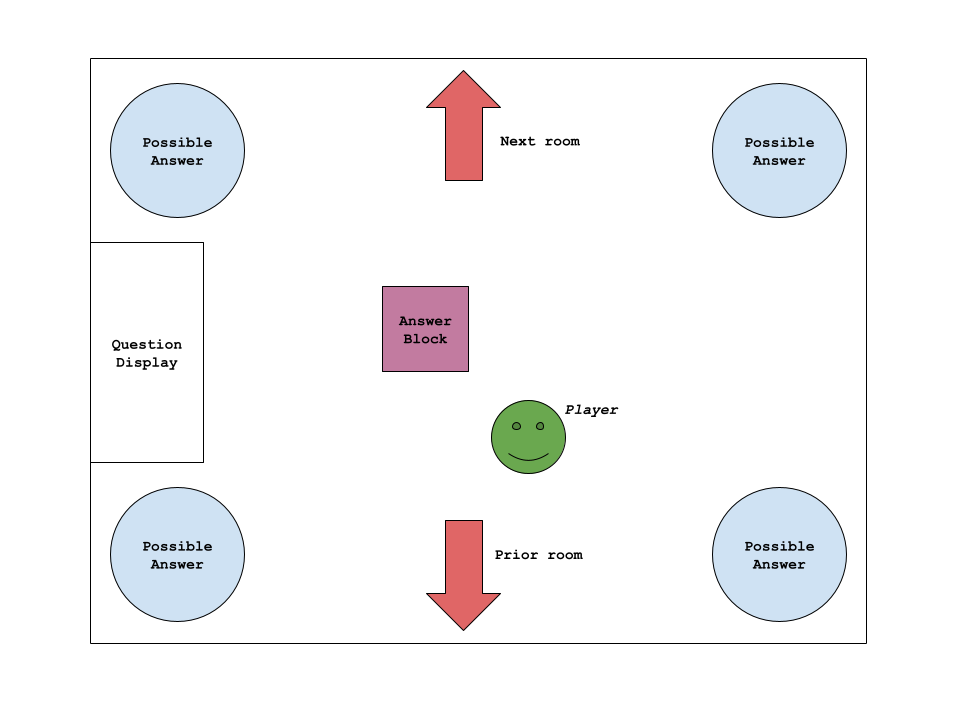
\includegraphics[width=\linewidth]{Demo.png}
 \caption{A concept design generated prior to the implementation of the project, this visualizes a top-down view of each "question room" within the environment. Some of the finer aspects were refined during implementation, but largely remain the same.}
 \label{fig:sample}
\end{figure}

The early prototype was capable of running a very early demo of the final product, as seen in Figure 3. The player character was fully controllable across two dimensions, and could maneuver throughout the provided environment at will. This player character was able to interact with objects by running into them, although specific implementation for grabbing or picking up items was still pending at the time. Much progress has been made since this progress checkpoint, as seen in Figure 4. Control of the player character was extended to include vertical movement (jumping), as well as the ability of the player character to interact with objects in the environment, specifically picking up certain objects. These objects move with the position of the player, not where the player is looking, forcing participants to put a lot of emphasis into their individual motion to move such objects, which include the aforementioned "answer cubes" required to answer questions.

\begin{figure}[tb]
 \centering 
 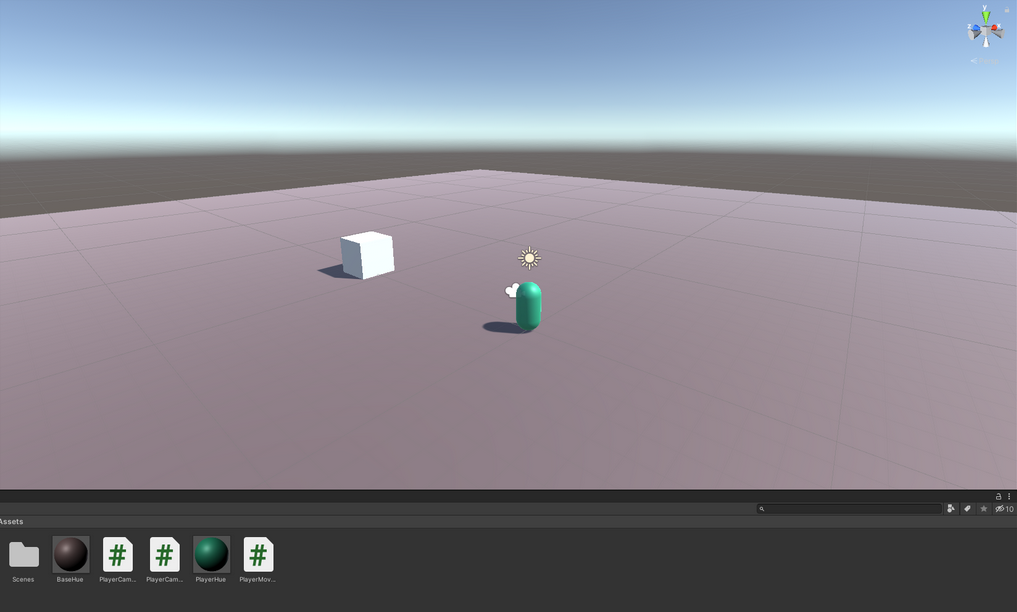
\includegraphics[width=\linewidth]{Prototype.png}
 \caption{Early visual from the prototype application; shows controllable-player character and a cube object on an empty plane.}
 \label{fig:sample}
\end{figure}

\begin{figure}[tb]
 \centering 
 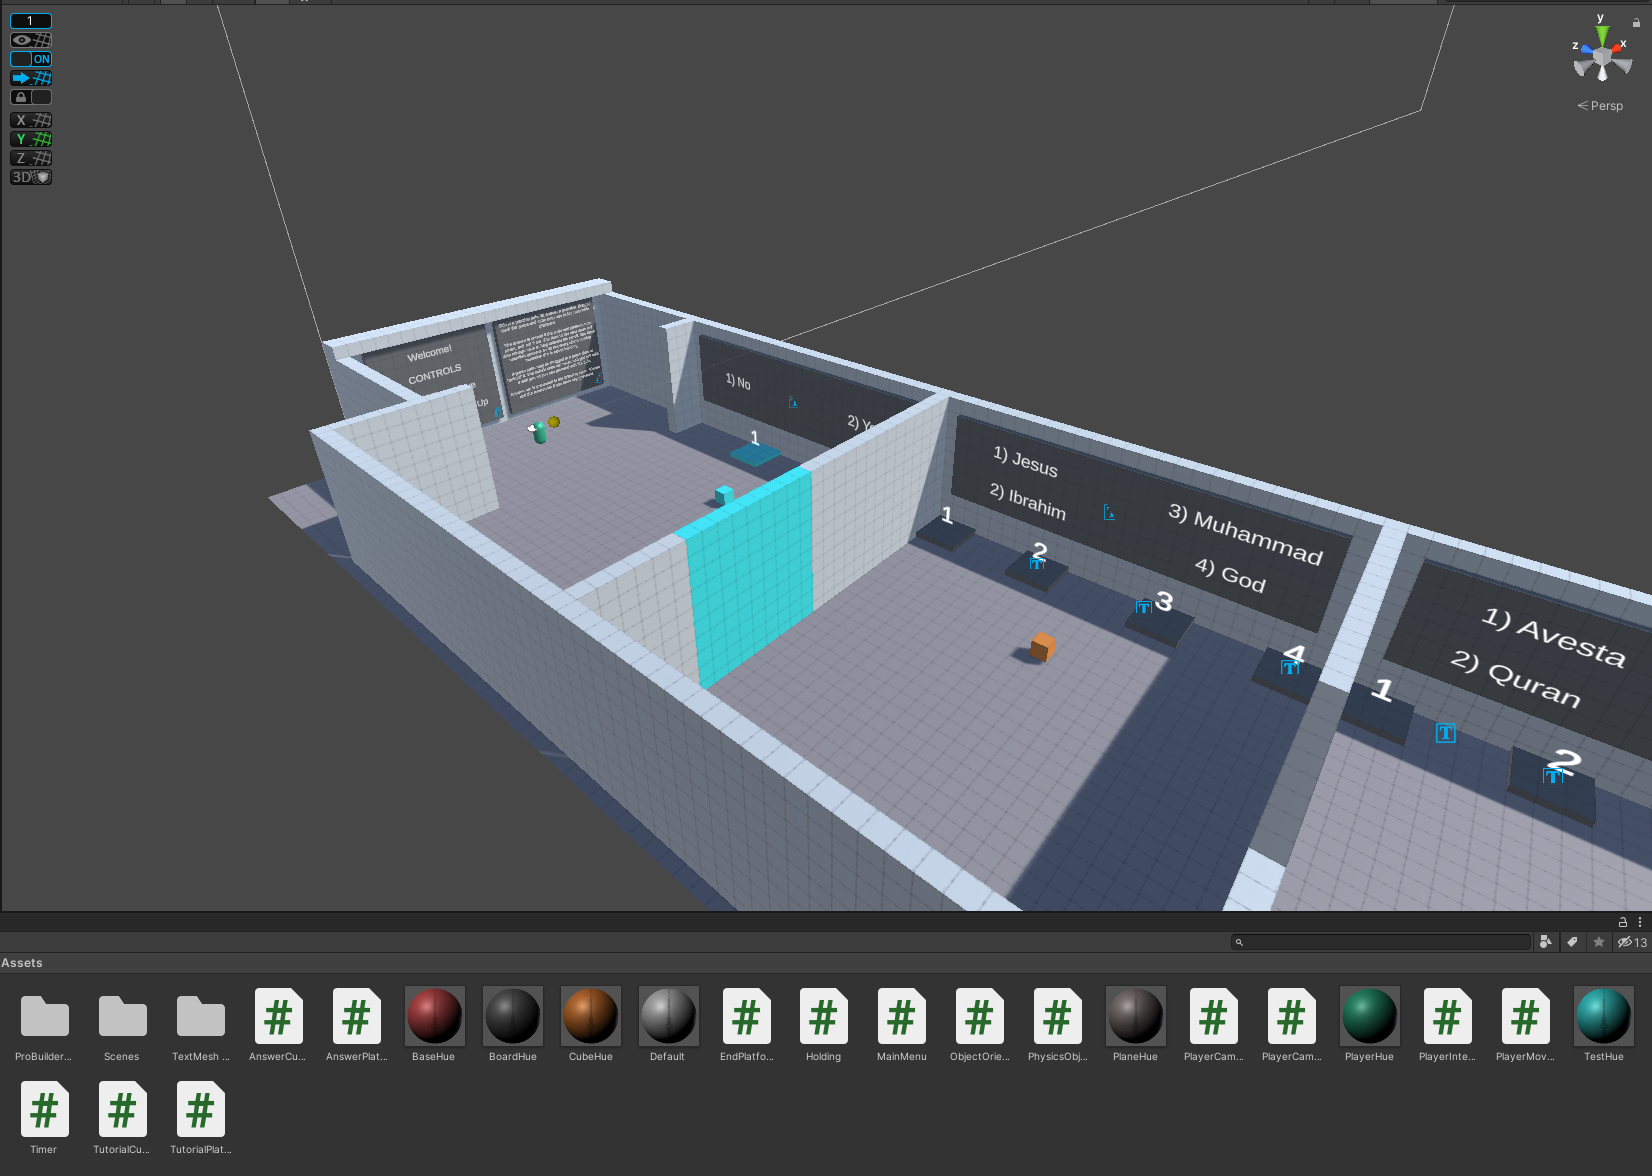
\includegraphics[width=\linewidth]{FinalPrototype.png}
 \caption{Visual of the final version of the prototype application, showing the player character staged for use in the tutorial area of the first level. The first "question room" is also visible, along with the "answer cube" used to progress through the level.}
 \label{fig:sample}
\end{figure}

While AR technology may have perhaps provided a stimulating medium for this research, the technical challenges presented by the development of an AR application were cause enough to shift the focus of this study to that of a virtual environment. While the experiment was still engineered within Unity, the 3D Core preset was used instead of the AR Core preset, and luckily allowed the initial plan to proceed mostly according to the original design. This transition came with many boons, as participants could use the latter format in any conceivable setting with a laptop or computer. This also avoided pitfalls around which specific settings the AR application was designed in, and if there would be issues with immersion if the room the application was used in changed and the virtual objects clipped through existing items within that space.

\section{Results and Discussion}

The primary statistical approach  used in the assessment of the prototype consists of an analysis of variance (ANOVA) test to determine the significance of both accuracy and time on performance within the software. A secondary and simple difference equation was used to determine net memorization of the content after exposure to the prototype. There were two major outliers in the dataset, as elaborated upon in the proceeding sections. No transformations or other types of data filtering occurred, all referenced within Table 1.

\subsection{Prototype}

\subsubsection{Accuracy}

Overall, the participants seemed to make about the same number of mistakes for each level of the prototype. The observed average task error for the first level participants completed was 5.88 and the standard deviation 2.64. The second completed level notably had a higher average error rate of 7.77 and a deviation of 2.57. The third level had an even higher mean error rate of 7.88 and standard deviation of 5.19. The effect of relative error on performance within the prototype was not statistically significant (F(2,16)=1.096, p=0.3579). Independent errors for each level of the prototype are visible in Table 1, and reveal a lot more variability in the number of mistakes participant made. It is important to note that for the third level the standard deviation was over twice as large as the other levels, indicating a lot more variability with the errors per each participant and skewing the results of the average error.

As evident in Figure 5, one major outlier presented itself here, with a participant producing a total number of 20 errors in Level 2. This is attributable to the fact that the participant made little to no use of the lecture sheet, intending to simply guess and learn for themselves throughout the study. However, this did not adversely affect their understanding of the content matter. In fact, another participant similarly noted that they did not require the lecture sheet and managed to produce one of the higher final quiz scores of the sample population despite scoring one of the lowest scores on the initial quiz without generating a relatively significant number of errors. There was one other minor outlier in the findings, with the respective participant generating errors of 12 and 11 in the first two levels, but again net memorization did not appear to be affected. This can perhaps be attributable to certain learning styles.

\begin{figure}[tb]
 \centering 
 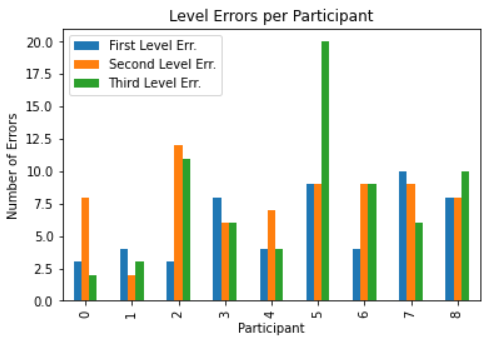
\includegraphics[width=\linewidth]{LevelErrorsParticipants.png}
 \caption{Total errors of each iterative level the participants completed according to their counterbalance.}
 \label{fig:sample}
\end{figure}

\begin{table}[tb]
 \centering 
 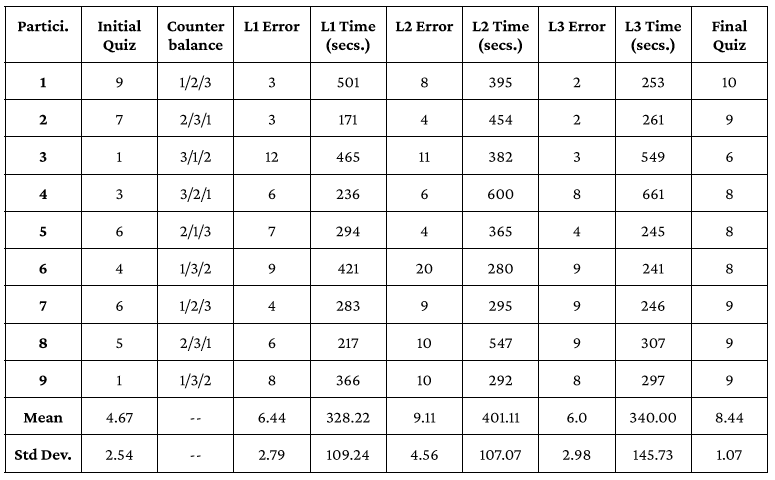
\includegraphics[width=\linewidth]{PerformanceTable.png}
 \caption{Full table of the generated output of each participant, according to their interactions with the prototype and the initial/final assessments.}
 \label{fig:sample}
\end{table}

One may initially think that errors would reduce as participants become more familiar with the prototype, but this average increase in error rate may actually be a result of familiarity as participants are more willing to take more risks and less cautious actions in an environment they have comfort in. Although, given warnings from Gros [3], errors may stem from complacency born of the "game-ification" of the learning process and the distortion of memorization with habits that influence a strictly logical way of thinking.

\subsubsection{Time}

Individual differences in time between each participant greatly varied. One participant felt the need to take upwards of ten minutes in a given level, while another only needed about two minutes. Despite this contrast the memorization of all participants appeared to benefit, as elaborated upon in a later subsection. The mean task completion time for first completed level of a participant was 460.77 seconds and a standard deviation of 109.70. The second level had a reduced average completion time at 350.55 seconds with a deviation of 109.73. The third completed level was even lower with an average time of 258.00 seconds and standard deviation of 54.86, indicating a lot more uniformity among the participants compared to the other levels. From this it can be inferred that participants grew increasingly familiar with the prototype as they completed successive levels. The effect of relative time on performance within the prototype was statistically significant (F(2,16)=15.625, p=.0002). Figure 6 visualizes this decline in time as the participants interact with the prototype.

\begin{figure}[tb]
 \centering 
 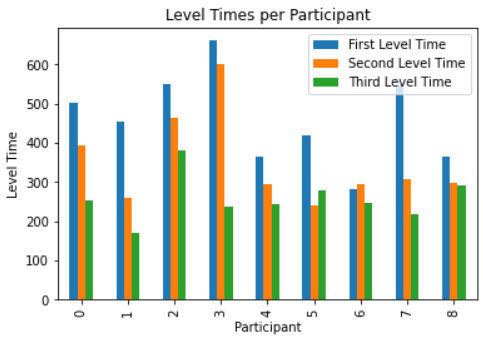
\includegraphics[width=\linewidth]{LevelTimesParticipants.png}
 \caption{Total time it took participants to complete successive levels in the prototype, according to their counterbalance.}
 \label{fig:sample}
\end{figure}

Independent participant times for each level of the prototype are likewise visible in Table 1. As each iterative level had arguably harder questions related to the content matter, it is understandable that the latter two levels would have higher completion times than the first, although the largely increased standard deviations indicate a lower uniformity across the sample population.

\subsubsection{Accuracy and Time}

When combining both accuracy and time, and accounting for the order users completed each level in, we see an average increase of 1.00 in relative errors and an average decrease in relative time of 67.59 seconds as participants progress through the study.

A rise in errors is seemingly contradictory to the findings of Ragan et al. [8], who found that even slight increases in user immersion were associated with significant increases in user task performance, and attribute this to enhanced spatial cues. 

\subsubsection{Feedback}

Most participants expressed a positive response to the prototype and seemed to really throw themselves into the content when introduced to the software, some expressing a few stunned verbal reactions upon loading into their first level. One participant said it was effective at memorization with content they did not know, but qualified that by asserting they knew most of the content already. Another expressed that if they could learn through video games (or virtual environments) a lot of aspects about education would be easier. A participant tested towards the end of the study even went so far as to suggest a control group to empirically see just how much of a better format this prototype was at memorization compared to more traditional methods, and hypothesized about how similar technologies might be used in the future. These latter two comments reference early ideas expressed by Squire [9] and the use of certain software simulations in educational environments. Of all the participants, hardly any needed to take breaks between levels, all expressing a high morale and motivation to learn the subject matter. This parallels the outcomes of Koutsabasis et al. [5] who all discovered that their students displayed increased engagement when presented with problem-based learning activities in a virtual environment.

\subsubsection{Noted Behaviors}

\paragraph{Mobility} Six of the participants were observed making a great extent of the mobility mechanics offered to them in the prototype. This included frequent use of the jumping mechanic, gaining elevation and maneuvering wildly in the air between and when answering questions. Participants who engaged in this behavior seemed to enjoy doing so, giving credence to the types of movement categories presented by Pasch et al. [7] and how they increase player immersion and emotional engagement. However, this did cause some concerns as several of these participants almost managed to navigate out of bounds of the levels through this behavior; so as not to inhibit player movement, a solution could perhaps be to implement a high ceiling across the whole level. Three of these six participants would physically go back through the level to review the answers to prior questions. These telltale signs of immersion are a positive sign, although for the sake of the study caused issues when a few participants rushed to complete a level without stopping to inform the present researcher. Overall these observations align with the findings of Ragan et al. [8], who found that even slight increases in user immersion were associated with significant increases in user task performance, and attribute this to enhanced spatial cues. The remaining three participants did not undertake as much personal experimentation with movement.

\paragraph{Interactivity} Participants took to the interactive nature of the prototype, but continually expressed certain struggles with the tentative nature of the answer cube. This specifically included the cube pushing the player when positioned incorrectly, and insisting on running into a given door while holding the cube instead of pushing the cube to the door. This extended to the answer platform, as all participants were observed to unnecessarily direct the cube to the end of each level. Without any direction some participants learned how to throw the cube and began to use that mechanic to launch it onto the answer platforms, although curiously did not use this same feature to open the door to the next question. This can perhaps be ascribed to associated with legacy bias from when initially learning the prototype. When the answer for a question was unclear or not provided on the lecture sheet, most of the participants resorted to a blind guessing tactic by randomly dropping the cube on the platforms until both turned green. While perhaps not ideal, the associated errors of these mistakes were displayed to each participant by responsive UI in the corner of the screen, stemming from ideas outlined in the report of Dyck et al. [2].

\paragraph{Confusion} Participant confusion largely stems from issues with the tutorial, as they fail to look around at the entire room once they begin their first level. This extends to the doors themselves; they were not initially clear to most of the participants, and besides behavior running into the doors, one participant forgot how to unlock the door entirely. These problems would likely be solved by a more in-depth or dedicated tutorial level. In other related inconsistencies, another participant reported the whole experience as overwhelming. The last participant, completely non-reliant on the lecture sheet and more prone to random guesses, discovered two of the thirty questions actually had two possible answers unlike other participants, and cited that as confusion for their answers on the final quiz.

\paragraph{Lecture Sheet} Only two of the nine participants wrote on their physical lecture sheets, while another two did not use their lecture sheet at all. Markings either consisted of simple underlines or very brief notes written on the back of the page. The remaining seven participants all made variable use of the lecture sheet depending on their overall confidence, but even the two participants who did not make use of the provided notes still excelled in the final quiz, earning an average of six points between them.

\subsection{Memorization}

\subsubsection{Initial Quiz}

There were a very wide range of scores on the initial quiz, as indicated by Figure 7. A significant outlier can immediately be seen with one participant, having scored a 9 out of 10 on the initial quiz and a 10 on the final quiz. This can be associated with their reported major (history) and expressed familiarity with Islam. The observed average mean initial score was 4.67 out of 10 with a standard deviation of 2.54 points. Seven of the ten questions on this quiz were commonly answered incorrect in three-to-four instances of the quiz, with the remaining three questions only being answered incorrectly 0-2 times. Referencing prior questionnaire responses, only three participants reported having familiarity with Islam thus giving an indicator for the low performance; this result is beneficial for the aim of testing the prototype however, as it indicates the utilized subject matter was relatively unknown to most of the sampled participants.

\begin{figure}[tb]
 \centering 
 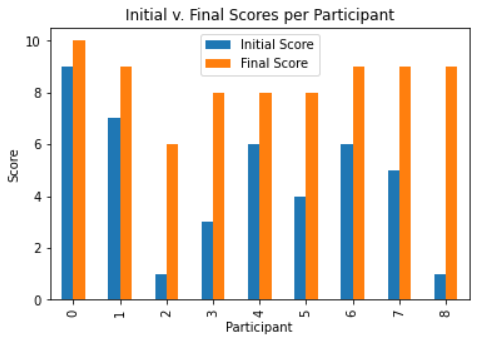
\includegraphics[width=\linewidth]{InitialFinalScores.png}
 \caption{The performance of each participant on the initial and final quizzes taken at the beginning and end of the study.}
 \label{fig:sample}
\end{figure}

\subsubsection{Final Quiz}

Contrasted to the initial quiz, final quiz scores were much more concise. The observed average mean final score was 8.44 out of 10 with a standard deviation of 1.07 points. Only one question was commonly answered incorrectly, four out of nine times, but is attributable to a previously identified error with two answers in the prototype. The average learning rate between all participants is a gain of 3.77 points, determined by averaging the point difference between the initial and final quizzes. The effect of exposure to the prototype to memorization was statistically significant (F(1,8)=28.900, p=.0007). Similar to previous research [1,6], these applications were successful in ensuring the memorization of the content matter despite largely minimal familiarity to it by the participants. And, unlike Hafner at al. [4], indicate that immersion within a virtual environment did in fact affect memorization, perhaps aided by the prototype's more accessible format.

\section{Conclusion}

A prototype was developed to research the effects of motion and immersion within a virtual environment on memorization. The test for the prototype was a 3x3 within-subjects design based on repeated measures with a counterbalance. Nine participants utilized this prototype to explore a random subject matter for the sake of testing its effectiveness by taking a series of simple practice quizzes within the virtual environment. The accuracy and completion time of each participant were measured for further analysis and the assessment of the significance of the experiment.

Findings include that exposure to the prototype and net memorization, along with the effect of time on performance within the prototype, are statistically significant. Contrarily, the effect of relative error (or accuracy) within the prototype was not found to be statistically significant.

The prototype and the research born of it will \textbf{contribute} to the field of computer-aided memorization, but more specifically to how individuals and groups can utilize said technology in study techniques and educational settings. This extends on prior work by scholars who wish to use computer technology to aid in the education of their religion [1,6] and of computer scientists and educators who recognize the possibilities presented by virtual environments for the use of skill learning [2, 7, 8] and content memorization [4, 5, 9] in modern work and school settings, all taking the pervasive nature of the format into consideration [3, 11].

Topics for further work primarily include further refinements to the prototype and the implementation of additional features, such as how audio cues effect or influence memorization, or testing how specific game mechanics influence and alter the learning processes of individuals. However, subsequent research does not need to be limited to the confines of this specific prototype.

%\bibliographystyle{abbrv-doi}
\bibliographystyle{plainurl}

\cite{src1} \cite{src2} \cite{src3} \cite{src4} \cite{src5}
\cite{src6} \cite{src7} \cite{src8} \cite{src9} \cite{src10}
\cite{quizlet}
\bibliography{refs}

\end{document}
